%%%%%%%%%%%%%%%%%%%%%%%%%%%%%%%%%%%%
% Slide options
%%%%%%%%%%%%%%%%%%%%%%%%%%%%%%%%%%%%

% Option 1: Slides with solutions

\documentclass[slidestop,compress,mathserif]{beamer}
\usepackage{booktabs}
\newcommand{\soln}[1]{\textit{#1}}
\newcommand{\solnGr}[1]{#1}

% Option 2: Handouts without solutions

%\documentclass[11pt,containsverbatim,handout]{beamer}
%\usepackage{pgfpages}
%\pgfpagesuselayout{4 on 1}[letterpaper,landscape,border shrink=5mm]
%\newcommand{\soln}[1]{ }
%\newcommand{\solnGr}{ }

%%%%%%%%%%%%%%%%%%%%%%%%%%%%%%%%%%%%
% Style
%%%%%%%%%%%%%%%%%%%%%%%%%%%%%%%%%%%%
%%%%%%%%%%%%%%%%%%%%%%%%%%%%%%%%%%%%%%%%%%%%%%%%%%%%%%%%%%%%%%%%%%%%%%%%
% MA213/214 shared slide style
%
% "Calm & Cool" palette + content-type callout boxes.
% Overhauled (2026) from the original OpenIntro/metropolis style:
%   - all OpenIntro visual branding removed (logo, grid, colors)
%   - a low-key cool palette (see colors below)
%   - tcolorbox callout boxes so students recognize content types
% See common/README.md for the command cheat-sheet.
%%%%%%%%%%%%%%%%%%%%%%%%%%%%%%%%%%%%%%%%%%%%%%%%%%%%%%%%%%%%%%%%%%%%%%%%

\usetheme{metropolis}

%%%%%%%%%%%%%%%%
% Packages
%%%%%%%%%%%%%%%%

\usepackage{geometry}
\usepackage{graphicx}
\usepackage{amssymb}
\usepackage{epstopdf}
\usepackage{amsmath}  	% this permits text in eqnarray among other benefits
\usepackage{url}		% produces hyperlinks
\usepackage{hyperref}	% allows for color usage in tables
\usepackage[english]{babel}
\usepackage[latin1]{inputenc}
\usepackage{colortbl}	% allows for color usage in tables
\usepackage{multirow}	% allows for rows that span multiple rows in tables
\usepackage{color}		% this package has a variety of color options
\usepackage{pgf}
\usepackage{calc}
\usepackage{ulem}
\usepackage{multicol}
\usepackage{textcomp}
\usepackage{txfonts}
\usepackage{listings}
\usepackage{tikz}
\usepackage{array}
\usepackage{wasysym}
\usepackage{fancyvrb}
\usepackage{etoolbox}             % \ifstrempty for optional box subtitles
\usepackage[most]{tcolorbox}      % content-type callout boxes
\tcbuselibrary{listings}          % R-code block (\begin{rblock})
\usepackage{fontawesome5}         % box icons

%%%%%%%%%%%%%%%%
% Remove navigation symbols
%%%%%%%%%%%%%%%%

\setbeamertemplate{navigation symbols}{}

%%%%%%%%%%%%%%%%
% "Calm & Cool" palette
%%%%%%%%%%%%%%%%

% chrome / structure / body
\definecolor{ccSlate}{HTML}{2E3742}   % frametitle bar, structure, section pages (deep neutral slate)
\definecolor{ccInk}{HTML}{2B2B2B}     % body text
\definecolor{ccWash}{HTML}{FCF8F1}    % gentle warm title-slide background wash (complements the cool blues)

% example (blue)
\definecolor{ccBlue}{HTML}{2F6690}
\definecolor{ccBlueBg}{HTML}{EAF1F7}
% interactive activity / discussion (green)
\definecolor{ccGreen}{HTML}{4E8A6B}
\definecolor{ccGreenBg}{HTML}{E9F3EC}
% solution (purple)
\definecolor{ccPurple}{HTML}{6F5499}
\definecolor{ccPurpleBg}{HTML}{EFEAF6}
% worksheet / focused work (terracotta)
\definecolor{ccTerra}{HTML}{C2693E}
\definecolor{ccTerraBg}{HTML}{FAEDE4}
% formula / definition (neutral slate)
\definecolor{ccGray}{HTML}{5C6B7A}
\definecolor{ccGrayBg}{HTML}{EEF1F4}
% caution / common pitfall (brick red)
\definecolor{ccRed}{HTML}{B23A48}
\definecolor{ccRedBg}{HTML}{FAEAEC}
% key idea / takeaway (muted gold)
\definecolor{ccGold}{HTML}{9C7A28}
\definecolor{ccGoldBg}{HTML}{F7F1DF}
% learning goals / lesson outcomes (teal)
\definecolor{ccTeal}{HTML}{2C6E6B}
\definecolor{ccTealBg}{HTML}{E6F0EF}
% learning objectives (indigo)
\definecolor{ccIndigo}{HTML}{45507A}
\definecolor{ccIndigoBg}{HTML}{ECEEF4}
% R code / output (gray)
\definecolor{ccCode}{HTML}{5F5E5A}
\definecolor{ccCodeBg}{HTML}{F4F5F6}

% neutral grays kept from the original style
\definecolor{gray}{rgb}{0.5, 0.5, 0.5}
\definecolor{darkGray}{rgb}{0.3, 0.3, 0.3}
\definecolor{darkerGray}{rgb}{0.2, 0.2, 0.2}

% Backwards-compatible aliases: old OpenIntro color names now point at the
% new palette, so existing \textcolor{oiB}{...}, \hl{...}, etc. keep working.
\colorlet{oiB}{ccBlue}
\colorlet{oiG}{ccGreen}
\colorlet{hlblue}{ccBlue}
\colorlet{rubineRed}{ccRed}
\colorlet{irishGreen}{ccGreen}
\colorlet{lightGreen}{ccGreen}

%%%%%%%%%%%%%%%%
% Restyle metropolis with the Calm & Cool chrome
%%%%%%%%%%%%%%%%

\metroset{block=fill}

\setbeamercolor{normal text}{fg=ccInk, bg=white}
\setbeamercolor{structure}{fg=ccSlate}
\setbeamercolor{alerted text}{fg=ccBlue}
\setbeamercolor{example text}{fg=ccGreen}
\setbeamercolor{frametitle}{bg=ccSlate, fg=white}
\setbeamercolor{progress bar}{fg=ccBlue}
\setbeamercolor{title separator}{fg=ccBlue}
\setbeamercolor{title}{fg=ccSlate}
\setbeamercolor{subtitle}{fg=ccBlue}
\setbeamercolor{author}{fg=ccInk}
\setbeamercolor{institute}{fg=ccGray}
\setbeamercolor{date}{fg=ccGray}
\setbeamercolor{section title}{fg=ccSlate}
\setbeamercolor{standout}{fg=white, bg=ccSlate}

% Section pages sit on the same warm wash as the title slide. We keep
% metropolis's section-title styling and just paint a full-page ccWash
% background behind it (needs >=2 pdflatex passes for the current-page node).
\setbeamertemplate{section page}{%
  \begin{tikzpicture}[remember picture, overlay]
    \fill[ccWash] (current page.south west) rectangle (current page.north east);
  \end{tikzpicture}%
  \centering
  \begin{minipage}{22em}
    \raggedright
    \usebeamercolor[fg]{section title}%
    \usebeamerfont{section title}%
    \insertsectionhead\\[-1ex]
    \usebeamertemplate*{progress bar in section page}%
    \par
  \end{minipage}\par
  \vspace{\baselineskip}
}

%%%%%%%%%%%%%%%%
% Custom inline text commands (recolored to the palette)
%%%%%%%%%%%%%%%%

% degree
\newcommand{\degree}{\ensuremath{^\circ}}

% cite
\newcommand{\ct}[1]{
\vfill
{\tiny #1}}

\newcommand{\NamedNote}[2]{
\rule{2.5cm}{0.25pt} \\ \textit{\footnotesize{\textcolor{rubineRed}{#1:} \textcolor{darkerGray}{#2}}}}

% Note
\newcommand{\Note}[1]{
\rule{2.5cm}{0.25pt} \\ \textit{\footnotesize{\textcolor{rubineRed}{Note:} \textcolor{darkerGray}{#1}}}}

% Remember
\newcommand{\Remember}[1]{\textit{\scriptsize{\textcolor{ccTerra}{Remember:} #1}}}

% expected counts
\newcommand{\ex}[1]{\textit{\textcolor{ccBlue}{#1}}}

% red
\newcommand{\red}[1]{\textit{\textcolor{rubineRed}{#1}}}

% pink
\newcommand{\pink}[1]{\textit{\textcolor{rubineRed!90!white!50}{#1}}}

% green
\newcommand{\green}[1]{\textit{\textcolor{irishGreen}{#1}}}

% orange
\newcommand{\orange}[1]{\textit{\textcolor{ccTerra}{#1}}}

% links: webURL, webLink, appLink
\newcommand{\webURL}[1]{\urlstyle{same}{ \textit{\textcolor{darkGray}{\url{#1}}}}}
\newcommand{\webLink}[2]{\href{#1}{\textcolor{darkGray}{{#2}}}}
\newcommand{\appLink}[2]{\href{#1}{\textcolor{white}{{#2}}}}

% mail
\newcommand{\mail}[1]{\href{mailto:#1}{\textit{\textcolor{darkGray}{#1}}}}

% highlighting: hl, hlGr, mathhl
\newcommand{\hl}[1]{\textit{\textcolor{hlblue}{#1}}}
\newcommand{\hlGr}[1]{\textit{\textcolor{lightGreen}{#1}}}
\newcommand{\mathhl}[1]{\textcolor{hlblue}{\ensuremath{#1}}}

%%%%%%%%%%%%%%%%
% Structural helpers (unchanged from the original)
%%%%%%%%%%%%%%%%

% two col: two columns
\newenvironment{twocol}[4]{
\begin{columns}[c]
\column{#1\textwidth}
#3
\column{#2\textwidth}
#4
\end{columns}
}

% slot (for probability calculations)
\newenvironment{slot}[2]{
\begin{array}{c}
\underline{#1} \\
#2
\end{array}
}

% pr: left and right parentheses
\newcommand{\pr}[1]{
\left( #1 \right)
}

% cancel
\newcommand{\cancel}[1]{%
    \tikz[baseline=(tocancel.base)]{
        \node[inner sep=0pt,outer sep=0pt] (tocancel) {#1};
        \draw[red, line width=0.5mm] (tocancel.south west) -- (tocancel.north east);
    }%
}

% removepagenumbers
\newcommand{\removepagenumbers}{%
  \setbeamertemplate{footline}{}
}

% change margin
\newenvironment{changemargin}[2]{%
\begin{list}{}{%
\setlength{\topsep}{0pt}%
\setlength{\leftmargin}{#1}%
\setlength{\rightmargin}{#2}%
\setlength{\listparindent}{\parindent}%
\setlength{\itemindent}{\parindent}%
\setlength{\parsep}{\parskip}%
}%
\item}{\end{list}}

% footnote
\long\def\symbolfootnote[#1]#2{\begingroup%
\def\thefootnote{\fnsymbol{footnote}}\footnote[#1]{#2}\endgroup}

% commands from the book
\newenvironment{data}[1]{\texttt{#1}}{}
\newenvironment{var}[1]{\texttt{#1}}{}
\newenvironment{resp}[1]{\texttt{#1}}{}

%%%%%%%%%%%%%%%%
% Content-type callout boxes (tcolorbox)
%
% Each type has a colored title strip (icon + label) over a light fill.
% Color = content type; the label + icon reinforce it (so the cue does
% not rely on color alone).
%%%%%%%%%%%%%%%%

\tcbset{
  cccallout/.style 2 args={
    enhanced, breakable=false,
    colback=#2, colframe=#1, colbacktitle=#1, coltitle=white,
    fonttitle=\bfseries\footnotesize,
    boxrule=0.6pt, arc=2.5pt, outer arc=2.5pt,
    left=5pt, right=5pt, top=3pt, bottom=3pt, boxsep=2pt,
    toptitle=2pt, bottomtitle=2pt, lefttitle=5pt,
    before skip=5pt, after skip=5pt,
  },
}

% One-off / collection of examples (blue): \workedexample[subtitle]{body}.
% (Named \workedexample, not \example, because beamer defines \example.)
\newtcolorbox{examplebox}[1][]{cccallout={ccBlue}{ccBlueBg},
  title={\faIcon{lightbulb}~~Example\ifstrempty{#1}{}{ \textmd{---}\ #1}}}
\newcommand{\workedexample}[2][]{\begin{examplebox}[#1]#2\end{examplebox}}

% Running-example header (blue): \examplehead{name} at the top of each frame of a
% multi-slide running example. A one-off or a collection of examples uses the
% \workedexample box above instead.
\newcommand{\examplehead}[1]{%
  \vspace{-0.4em}\par\noindent\tcbox[on line, colback=ccBlue, colframe=ccBlue, coltext=white,
    boxrule=0pt, arc=2pt, left=5pt, right=5pt, top=1pt, bottom=1pt,
    box align=base, nobeforeafter]{\footnotesize\bfseries\faIcon{lightbulb}\,Running example}%
  \ifstrempty{#1}{}{\enspace{\footnotesize\bfseries\textcolor{ccBlue}{#1}}}%
  \par\nobreak\vspace{-0.6em}{\color{ccBlue}\rule{\linewidth}{0.7pt}}\par\nobreak\vspace{-0.8em}}

% Interactive activity (green): \activity[subtitle]{body}
\newtcolorbox{activitybox}[1][]{cccallout={ccGreen}{ccGreenBg},
  title={\faIcon{users}~~Activity\ifstrempty{#1}{}{ #1}}}
\newcommand{\activity}[2][]{\begin{activitybox}[#1]#2\end{activitybox}}

% Discussion question (green): \dq{body}
\newtcolorbox{dqbox}{cccallout={ccGreen}{ccGreenBg}, title={\faIcon{comments}~~Discussion}}
\newcommand{\dq}[1]{\begin{dqbox}#1\end{dqbox}}

% Solution (purple): \solnbox{body}. Gated by the per-deck \soln toggle, so it
% shows in the instructor build and vanishes from the student handout build.
% (Named \solnbox, not \solution, because beamer already defines \solution.)
\newtcolorbox{solutionbox}{cccallout={ccPurple}{ccPurpleBg}, title={\faIcon{key}~~Solution}}
\newcommand{\solnbox}[1]{\soln{\begin{solutionbox}#1\end{solutionbox}}}

% Worksheet / focused work (terracotta): \worksheet[subtitle]{body}
\newtcolorbox{worksheetbox}[1][]{cccallout={ccTerra}{ccTerraBg},
  title={\faIcon{pencil-alt}~~Worksheet\ifstrempty{#1}{}{ #1}}}
\newcommand{\worksheet}[2][]{\begin{worksheetbox}[#1]#2\end{worksheetbox}}

% Formula / definition (neutral slate). Supports both real usages found in the
% decks: \formula{title}{body} and the bare \formula{body} (title defaults to
% "Formula"). The second group is an optional brace argument.
\newtcolorbox{formulabox}[1][Formula]{cccallout={ccGray}{ccGrayBg},
  title={\faIcon{square-root-alt}~~#1}}
\NewDocumentCommand{\formula}{m g}{%
  \IfNoValueTF{#2}%
    {\begin{formulabox}#1\end{formulabox}}%
    {\begin{formulabox}[#1]#2\end{formulabox}}}

% Common pitfall / caution (brick red): \caution[subtitle]{body}
\newtcolorbox{cautionbox}[1][]{cccallout={ccRed}{ccRedBg},
  title={\faIcon{exclamation-triangle}~~Caution\ifstrempty{#1}{}{ #1}}}
\newcommand{\caution}[2][]{\begin{cautionbox}[#1]#2\end{cautionbox}}

% Key idea / takeaway (muted gold): \keyidea[subtitle]{body}
\newtcolorbox{keyideabox}[1][]{cccallout={ccGold}{ccGoldBg},
  title={\faIcon{star}~~Key idea\ifstrempty{#1}{}{ #1}}}
\newcommand{\keyidea}[2][]{\begin{keyideabox}[#1]#2\end{keyideabox}}

% Learning goals / lesson outcomes (teal): \goals{body}. Sits under the short
% LO headings on the objectives slide; body is the "you should be able to" list.
\newtcolorbox{goalsbox}{cccallout={ccTeal}{ccTealBg}, fontupper=\footnotesize,
  top=1pt, bottom=2pt, boxsep=1pt, before skip=3pt,
  title={\faIcon{bullseye}~~By the end of today, you should be able to\ldots}}
\newcommand{\goals}[1]{\begin{goalsbox}#1\end{goalsbox}}

% Learning objectives (indigo): \objectives{body} -- the formal LO headings,
% shown alongside \goals on the objectives slide.
\newtcolorbox{objectivesbox}{cccallout={ccIndigo}{ccIndigoBg}, fontupper=\small,
  top=1pt, bottom=2pt, boxsep=1pt, before skip=3pt,
  title={\faIcon{clipboard-list}~~Learning objectives}}
\newcommand{\objectives}[1]{\begin{objectivesbox}#1\end{objectivesbox}}

% Defaults for a bare \begin{lstlisting}. Without these it inherits the listings
% package defaults: 11pt type, fixed-width columns (which spaces code out as
% "a g e _ f i t"), and no line breaking, so a long line silently runs off the
% right edge of the slide. A deck that passes its own basicstyle still wins.
% Layout only -- syntax coloring is left to the \begin{rblock} environment.
\lstset{
  basicstyle=\ttfamily\footnotesize, columns=fullflexible,
  breaklines=true, breakindent=1.5em, showstringspaces=false,
  numbers=none, frame=none}

% R code / output (gray): \begin{rblock}[subtitle] ... \end{rblock}
% NOTE: a frame containing an rblock must be declared \begin{frame}[fragile].
\lstdefinestyle{ccR}{
  language=R, basicstyle=\ttfamily\footnotesize, columns=fullflexible,
  breaklines=true, showstringspaces=false, numbers=none, frame=none,
  keywordstyle=\color{ccBlue}, commentstyle=\color{ccGreen!75!black},
  stringstyle=\color{ccTerra}}
\newtcblisting{rblock}[1][]{cccallout={ccCode}{ccCodeBg},
  title={\faIcon{terminal}~~R\ifstrempty{#1}{}{ #1}},
  listing only, listing style=ccR}

% --- Legacy boxes (kept so existing decks compile) ---

% app: application exercise -> alias of activity
\newcommand{\app}[1]{\activity{#1}}

% pq: practice question (green, interactive family)
\newtcolorbox{pqbox}{cccallout={ccGreen}{ccGreenBg}, title={\faIcon{list-ol}~~Practice}}
\newcommand{\pq}[1]{\begin{pqbox}#1\end{pqbox}}

% solnMult: solutions for multiple-choice practice questions (uses \soln toggle)
\newcommand{\solnMult}[1]{
\item[] \vspace{-0.59cm}
\only<1>{\item #1}
\soln{\only<2->{\item \orange{#1}}}
}

%%%%%%%%%%%%%%%%
% De-branded title frame + attribution
%%%%%%%%%%%%%%%%

% Eyebrow line on the title slide; a deck may \renewcommand this.
\newcommand{\coursetag}{MA214: Applied Statistics}

% Attribution: all slides released under CC BY-SA, crediting both the
% instructor (later material) and OpenIntro (basis of the earlier material).
\newcommand{\courseattribution}{%
  Slides by Jonathan H.~Huggins, building on materials from OpenIntro's
  \emph{Introduction to Modern Statistics} (Mine \c{C}etinkaya-Rundel et al.).
  Released under the
  \webLink{http://creativecommons.org/licenses/by-sa/3.0/us/}{CC BY-SA license}.
  Some images included under fair use (educational purposes).}

% \maketitleframe: de-branded title slide (no logo, no grid). Uses the deck's
% \title, \subtitle, and \coursetag.
\newcommand{\maketitleframe}{%
  \addtocounter{framenumber}{-1}%
  {\removepagenumbers
  \setbeamercolor{background canvas}{bg=ccWash}%
  \begin{frame}[plain]
    \vspace*{2.6em}
    {\color{ccSlate}\rule{\textwidth}{2.5pt}}\par\vspace{1.5em}
    {\usebeamerfont{date}\scshape\color{ccGray}\coursetag}\par\vspace{0.55em}
    {\usebeamerfont{title}\color{ccSlate}\inserttitle\par}
    \vspace{0.45em}{\color{ccBlue}\rule{3em}{2.5pt}}\par\vspace{0.7em}
    {\usebeamerfont{subtitle}\color{ccBlue}\insertsubtitle\par}
    \vfill
    {\color{ccGray!55}\rule{\textwidth}{0.4pt}}\par\vspace{0.45em}
    {\tiny\color{ccGray}\courseattribution\par}
    \vspace*{0.4em}
  \end{frame}}}

%%%%%%%%%%%%%%%%
% Graphics
%%%%%%%%%%%%%%%%

\DeclareGraphicsRule{.tif}{png}{.png}{`convert #1 `dirname #1`/`basename #1 .tif`.png}

\graphicspath{ {../../common/} {figures/}  }


%%%%%%%%%%%%%%%%%%%%%%%%%%%%%%%%%%%%
% Preamble
%%%%%%%%%%%%%%%%%%%%%%%%%%%%%%%%%%%%

\title[Lecture 12]{Lecture 12: Analysis of variance}
\subtitle{Module 2: Statistical Inference}
\author{Introduction to Modern Statistics, 2nd Edition}
\institute{$\:$ \\ {\footnotesize Based on slides developed by Mine \c{C}etinkaya-Rundel of OpenIntro.  \\
The slides may be copied, edited, and/or shared via the \webLink{http://creativecommons.org/licenses/by-sa/3.0/us/}{CC BY-SA license.} \\
Some images may be included under fair use guidelines (educational purposes).}}
\date{}

%%%%%%%%%%%%%%%%%%%%%%%%%%%%%%%%%%%%
% Begin document
%%%%%%%%%%%%%%%%%%%%%%%%%%%%%%%%%%%%

\begin{document}


%%%%%%%%%%%%%%%%%%%%%%%%%%%%%%%%%%%%
% Title page
%%%%%%%%%%%%%%%%%%%%%%%%%%%%%%%%%%%%

\maketitleframe



% !TEX root =  Lecture13.tex


%%%%%%%%%%%%%%%%%%%%%%%%%%%%%%%%%%%%
% Recap/Agenda
%%%%%%%%%%%%%%%%%%%%%%%%%%%%%%%%%%%%
\begin{frame}
\frametitle{Module 2: Statistical Inference}
    \begin{itemize}
        \item \hl{Previously:} two \emph{categorical} variables: two-way tables, expected counts, and the $\chi^2$ statistic.
        \item \hl{This time:} back to \emph{numbers}, but now \hl{three or more groups} of them.
          \begin{itemize}
              \item why running every pairwise $t$-test is a trap;
              \item one statistic for $k$ groups: variability \emph{between} the groups over variability \emph{within} them, the $F$-statistic;
              \item its null distribution, the same two ways: shuffle the group labels, or use the $F$ model;
              \item the conditions, and which road survives when they fail;
              \item after a significant $F$: \emph{which} groups actually differ?
          \end{itemize}
        \item \hl{Reading:} IMS Chapter 22.
        \item \hl{Homework for today:}
        \item \hl{Homework for next class:}
    \end{itemize}
\end{frame}


%%%%%%%%%%%%%%%%%%%%%%%%%%%%%%%%%%%%
% Learning objectives:
%%%%%%%%%%%%%%%%%%%%%%%%%%%%%%%%%%%%
\begin{frame}
    \frametitle{Lecture Objectives}
    \goals{%
    \begin{itemize}
    \item explain why testing every pair inflates the false-positive rate, and what a single simultaneous test buys you;
    \item split the total variability into a \emph{between-group} and a \emph{within-group} part, and build $F$ out of them;
    \item obtain $F$'s null distribution by \emph{shuffling the group labels} \textbf{and} from the $F_{df_1, df_2}$ model, and explain why they agree;
    \item check the conditions (normality, and above all \emph{equal variances}), and know which road survives when they fail;
    \item after a significant $F$, say \emph{which} groups differ without walking back into the trap you started with.
    \end{itemize}}
    \objectives{%
    \begin{itemize}
    \item \textbf{(M2, LO3)} Analysis of Variance (ANOVA)
    \end{itemize}}
\end{frame}


\section{The multiple-comparisons problem}

%%%%%%%%%%%%%%%%%%%%%%%%%%%%%%%%%%%%%%%%%%%%%%%%%%%%%%%%%%%%%%%%%%%%%%%%
\begin{frame}
\frametitle{Three or more groups of numbers}

\pause
\begin{itemize}\setlength{\itemsep}{2pt}
\item \textbf{Fertilizer and yield:} do four fertilizers give different mean yields?
\item \textbf{Class and vocabulary:} does vocabulary score depend on social class?
\item \textbf{Plot and weight:} does a kangaroo rat's weight depend on its plot type?
\end{itemize}

\pause
{\small The third is Lecture 11's Portal experiment with a new outcome: there a \emph{count} (which species?), here a \emph{number} (how heavy?).}

\pause
\dq{With $k$ groups, why not just run a $t$-test on every pair?}

\end{frame}


%%%%%%%%%%%%%%%%%%%%%%%%%%%%%%%%%%%%%%%%%%%%%%%%%%%%%%%%%%%%%%%%%%%%%%%%
\begin{frame}
\frametitle{The problem with many pairwise tests}

With $k$ groups there are $\binom{k}{2} = \frac{k(k-1)}{2}$ pairs to compare.

\pause
\vspace{0.3em}
Even if \emph{every} null hypothesis is true, each test still has probability $\alpha$ of a Type~I error. You only need \emph{one} of them to fire to be misled.

\pause
\vspace{0.3em}
\hl{If the tests were independent:}
\begin{align*}
P(\text{at least one Type I error})
&= 1 - P(\text{no Type I errors})  \\
&= 1 - P(\text{none on a given pair})^{\binom{k}{2}}  \\
&= 1 - (1 - \alpha)^{k(k-1)/2}.
\end{align*}

\end{frame}


%%%%%%%%%%%%%%%%%%%%%%%%%%%%%%%%%%%%%%%%%%%%%%%%%%%%%%%%%%%%%%%%%%%%%%%%
\begin{frame}
\frametitle{How fast does it grow?}

At $\alpha = 0.05$, with $1 - (1 - \alpha)^{k(k-1)/2}$:

\vspace{-0.2em}
\begin{center}
{\small
\begin{tabular}{ccc}
\toprule
Groups ($k$) & Pairs & $P(\text{at least one false rejection})$ \\
\midrule
3 & 3 & $1 - .95^{3} = 0.14$ \\
4 & 6 & $1 - .95^{6} = 0.26$ \\
5 & 10 & $1 - .95^{10} = 0.40$ \\
6 & 15 & $1 - .95^{15} = 0.54$ \\
\bottomrule
\end{tabular}}
\end{center}

\pause
\vspace{0.2em}
With six groups it is a \hl{coin flip} whether you report a difference that is not there.

\pause
\keyidea{Do not ask $\binom{k}{2}$ questions. Ask \emph{one}: \hl{are all $k$ means equal?} One test, one $\alpha$, one error rate. That test is \hl{ANOVA}.}

\end{frame}



\section{One number for $k$ groups}

%%%%%%%%%%%%%%%%%%%%%%%%%%%%%%%%%%%%%%%%%%%%%%%%%%%%%%%%%%%%%%%%%%%%%%%%
\begin{frame}
\frametitle{Analysis of Variance}

\textbf{AN}alysis \textbf{O}f \textbf{VA}riance (ANOVA) asks a single question about all $k$ groups at once:

\begin{itemize}
\item $H_0$: $\mu_1 = \mu_2 = \cdots = \mu_k$ \quad (all group means are equal)
\item $H_A$: at least one $\mu_i$ differs from the others
\end{itemize}

\pause
Note what $H_A$ does \emph{not} say: not which group, nor in which direction.

\pause
\keyidea[-- and where the name comes from]{To decide whether the means differ, look at \emph{variances}: compare the variability \hl{between} the group means with the variability \hl{within} them. Large gaps \emph{relative to the scatter inside the groups} mean the means are not all equal.}

\end{frame}


%%%%%%%%%%%%%%%%%%%%%%%%%%%%%%%%%%%%%%%%%%%%%%%%%%%%%%%%%%%%%%%%%%%%%%%%
\begin{frame}
\frametitle{Why it must be a \emph{ratio}}

\vspace{-0.3em}
\begin{center}
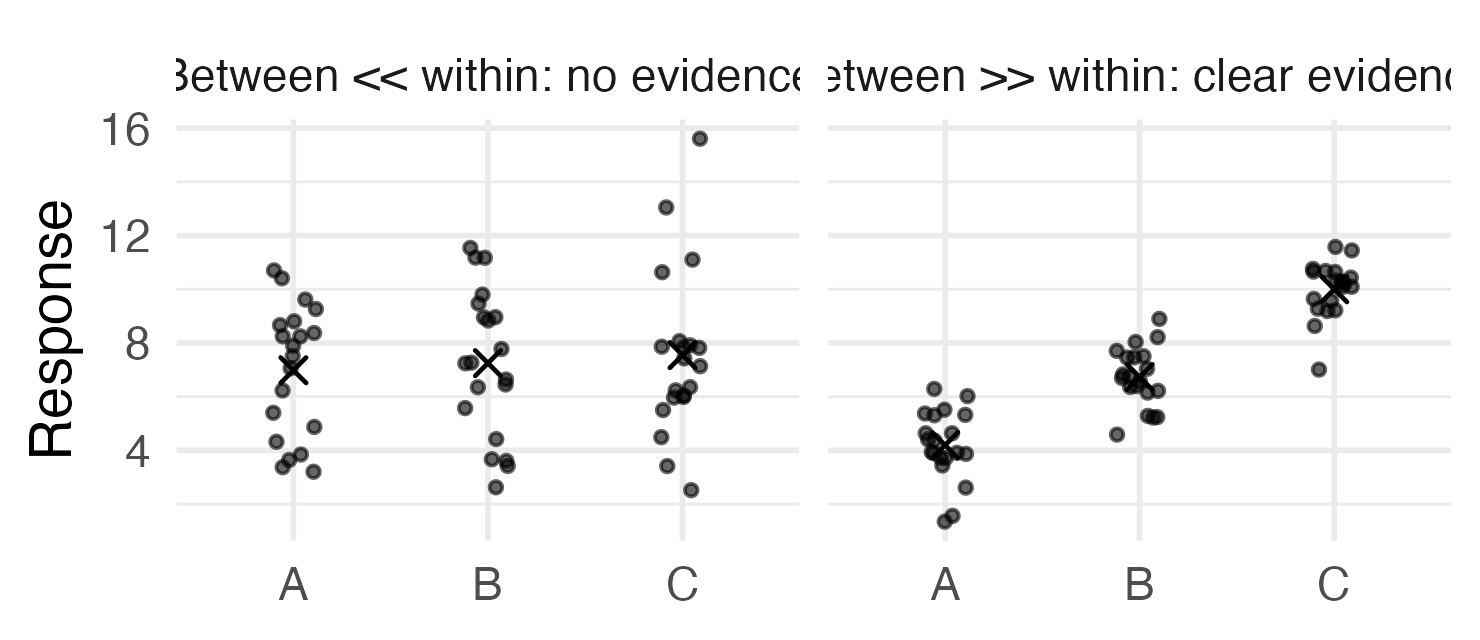
\includegraphics[width=0.8\textwidth]{anova_variability.png}
\end{center}

\vspace{-0.4em}
{\small Both panels have the \emph{same} three group means. Only the scatter within each group changes.}

\pause
\dq{Which panel is stronger evidence that the true means differ, and why can't you tell from the group means alone?}

\end{frame}


%%%%%%%%%%%%%%%%%%%%%%%%%%%%%%%%%%%%%%%%%%%%%%%%%%%%%%%%%%%%%%%%%%%%%%%%
\begin{frame}
\frametitle{Running example: 30 plants, 3 conditions}

\texttt{PlantGrowth} (Dobson, 1983): dried weight of plants grown under a control and two different treatments. $n = 30$, ten plants per group.

\vspace{-0.2em}
\begin{center}
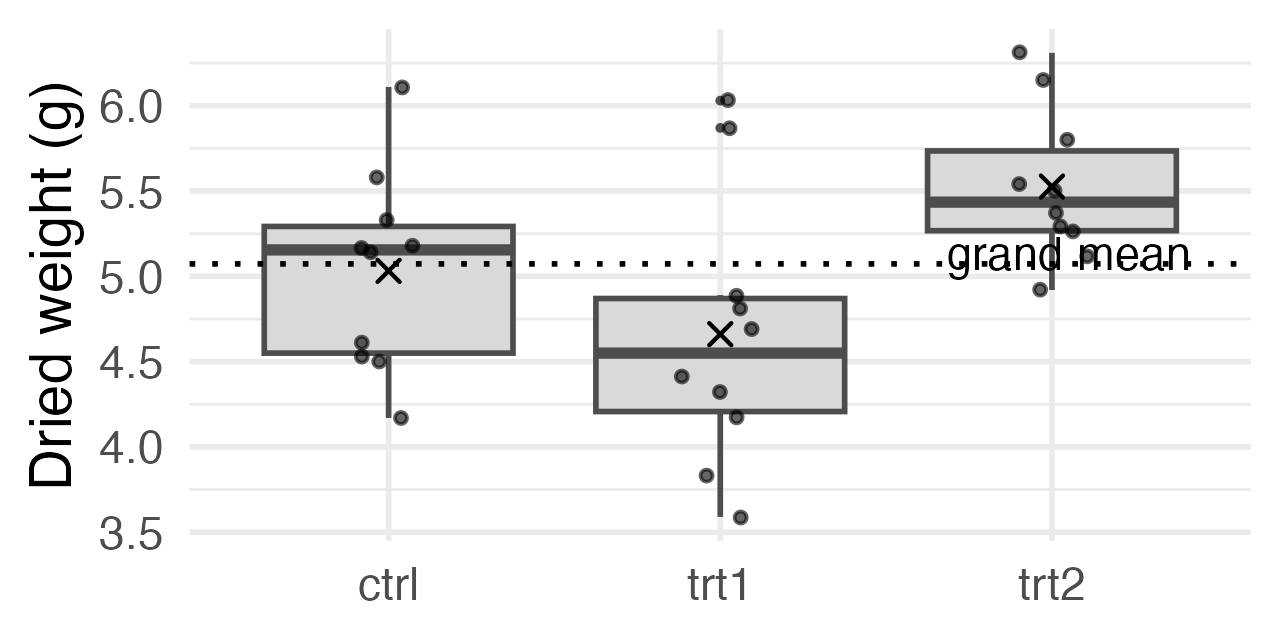
\includegraphics[width=0.72\textwidth]{plantgrowth_box.png}
\end{center}

\vspace{-0.4em}
{\small Group means: \texttt{ctrl} $5.03$, \texttt{trt1} $4.66$, \texttt{trt2} $5.53$ g. They differ, but the groups overlap heavily. Is $0.87$ g between \texttt{trt1} and \texttt{trt2} more than the scatter can explain?}

\end{frame}


%%%%%%%%%%%%%%%%%%%%%%%%%%%%%%%%%%%%%%%%%%%%%%%%%%%%%%%%%%%%%%%%%%%%%%%%
\begin{frame}
\frametitle{Measuring the two kinds of variability}

\formula{Sums of squares}{$\bar{x}_i$ is the mean of group $i$ (with $n_i$ observations) and $\bar{x}$ is the \emph{grand} mean of all $n$ points.
\[
\underbrace{SSG = \sum_{i=1}^{k} n_i\,(\bar{x}_i - \bar{x})^2}_{\text{\hl{between} the groups}}
\qquad
\underbrace{SSE = \sum_{i=1}^{k}\sum_{j=1}^{n_i} (x_{ij} - \bar{x}_i)^2}_{\text{\hl{within} the groups}}
\]}

\pause
\vspace{0.2em}
{\small \textbf{$SSG$} asks how far each \emph{group mean} sits from the grand mean, weighted by $n_i$, because a mean built from more plants counts for more.}

\pause
{\small \textbf{$SSE$} asks how far each \emph{plant} sits from its own group's mean. It is the scatter that has nothing to do with the treatment.}

\end{frame}


%%%%%%%%%%%%%%%%%%%%%%%%%%%%%%%%%%%%%%%%%%%%%%%%%%%%%%%%%%%%%%%%%%%%%%%%
\begin{frame}
\frametitle{The two parts add up}

Total variability about the grand mean splits cleanly in two:
\[
\underbrace{\sum_{i,j} (x_{ij} - \bar{x})^2}_{SST}
\;=\;
\underbrace{\sum_i n_i (\bar{x}_i - \bar{x})^2}_{SSG}
\;+\;
\underbrace{\sum_{i,j} (x_{ij} - \bar{x}_i)^2}_{SSE}
\]
\pause
\vspace{0.3em}
Each piece carries its own \hl{degrees of freedom}, and those add up too:

\vspace{0.2em}
\begin{center}
{\small
\begin{tabular}{lcl}
\toprule
 & $df$ & why \\
\midrule
$SSG$ & $k - 1$ & $k$ group means, minus 1 for the grand mean \\
$SSE$ & $n - k$ & $n$ points, minus 1 for each group mean \\
\midrule
$SST$ & $n - 1$ & $(k-1) + (n-k)$ \\
\bottomrule
\end{tabular}}
\end{center}

\pause
\vspace{0.2em}
{\small For the plants: $df_1 = 3 - 1 = 2$ and $df_2 = 30 - 3 = 27$.}

\end{frame}


%%%%%%%%%%%%%%%%%%%%%%%%%%%%%%%%%%%%%%%%%%%%%%%%%%%%%%%%%%%%%%%%%%%%%%%%
\begin{frame}
\frametitle{The $F$-statistic}

A sum of squares built from more pieces is naturally bigger, so divide each by its degrees of freedom first. That gives a \hl{mean square}, a variance.

\formula{The $F$-statistic}{
\[
F \;=\; \frac{MSG}{MSE} \;=\; \frac{SSG / (k-1)}{SSE / (n-k)}
\;=\; \frac{\text{variability \hl{between} the groups}}{\text{variability \hl{within} the groups}}
\]}

\pause
{\small Under $H_0$ the treatment does nothing, so numerator and denominator estimate the \emph{same} background variance and their ratio lands near \hl{$1$}. A large $F$ means the groups sit further apart than their internal scatter allows, so only large $F$ is evidence (the test is one-sided).}

\end{frame}


%%%%%%%%%%%%%%%%%%%%%%%%%%%%%%%%%%%%%%%%%%%%%%%%%%%%%%%%%%%%%%%%%%%%%%%%
\begin{frame}
\frametitle{The whole calculation, on 30 plants}
\examplehead{PlantGrowth}

Grand mean $\bar{x} = 5.073$. Group means $5.032$, $4.661$, $5.526$, ten plants each.

\vspace{0.2em}
{\small
\[
SSG = 10\big[(5.032 - 5.073)^2 + (4.661 - 5.073)^2 + (5.526 - 5.073)^2\big] = \hl{3.766}
\]}

\vspace{-0.6em}
{\small
\[
SSE = \sum_{i,j}(x_{ij} - \bar{x}_i)^2 = \hl{10.492}
\qquad (SST = 14.258 = 3.766 + 10.492 \;\checkmark)
\]}

\pause
\vspace{-0.2em}
{\small
\[
MSG = \frac{3.766}{2} = 1.883
\quad
MSE = \frac{10.492}{27} = 0.389
\quad
F_{\mathrm{obs}} = \frac{1.883}{0.389} = \hl{4.85}
\]}

\pause
\vspace{0.1em}
{\small \hl{Is $4.85$ far from $1$?} We cannot say yet: we need $F$'s null distribution.}

\end{frame}


%%%%%%%%%%%%%%%%%%%%%%%%%%%%%%%%%%%%%%%%%%%%%%%%%%%%%%%%%%%%%%%%%%%%%%%%
\begin{frame}[fragile]
\frametitle{And R agrees}
\examplehead{PlantGrowth}

\begin{lstlisting}[language=R, basicstyle=\ttfamily\scriptsize]
fit <- aov(weight ~ group, data = plants)
summary(fit)

            Df Sum Sq Mean Sq F value Pr(>F)
group        2  3.766  1.8832   4.846 0.0159 *
Residuals   27 10.492  0.3886
\end{lstlisting}

\vspace{-0.2em}
{\small Every number on the last slide is in this table: \texttt{Sum Sq} is $SSG$ and $SSE$; \texttt{Mean Sq} is $MSG$ and $MSE$; \texttt{Df} is $2$ and $27$. \texttt{Residuals} is R's name for ``within''.}

\pause
\vspace{0.2em}
{\small R also reports $\Pr(>F) = 0.0159$. \hl{Where does that come from?}}

\end{frame}


\section{Two roads to the null distribution}

%%%%%%%%%%%%%%%%%%%%%%%%%%%%%%%%%%%%%%%%%%%%%%%%%%%%%%%%%%%%%%%%%%%%%%%%
\begin{frame}
\frametitle{Road A: shuffle the group labels}
\examplehead{PlantGrowth}

To find out what $F$ looks like \emph{when $H_0$ is true}, impose $H_0$ on the data by force.

\pause
\keyidea[-- exchangeability]{If the growing condition truly has no effect, a plant's weight had nothing to do with its label, so that weight could equally well have carried \emph{any} of the three labels. The labels are \hl{exchangeable}.}

\pause
\vspace{-0.1em}
{\small
\begin{enumerate}
\item Keep the 30 weights as they are. \hl{Shuffle} the 30 group labels among them.
\item Recompute $F$.
\item Repeat $10{,}000$ times. That spread of $F$-values \emph{is} the null distribution.
\end{enumerate}}

\end{frame}


%%%%%%%%%%%%%%%%%%%%%%%%%%%%%%%%%%%%%%%%%%%%%%%%%%%%%%%%%%%%%%%%%%%%%%%%
\begin{frame}[fragile]
\frametitle{Road A in R}
\examplehead{PlantGrowth}

\begin{lstlisting}[language=R, basicstyle=\ttfamily\scriptsize]
# f_stat(y, g): the ANOVA F-statistic for response y, labels g
f_obs <- f_stat(plants$weight, plants$group)      # 4.85

null <- replicate(10000,
  f_stat(plants$weight, sample(plants$group)))     # shuffle!

mean(null >= f_obs)                                #> 0.0167
\end{lstlisting}

\vspace{-0.2em}
{\small \texttt{sample()} deals the labels out again at random; everything else is unchanged. The p-value is one-sided by construction: only \emph{large} $F$ is evidence, because $F$ cannot go below zero.}

\pause
\vspace{0.3em}
{\small So the randomization p-value is \hl{$0.0167$}.}

\end{frame}


%%%%%%%%%%%%%%%%%%%%%%%%%%%%%%%%%%%%%%%%%%%%%%%%%%%%%%%%%%%%%%%%%%%%%%%%
\begin{frame}
\frametitle{Road B: a formula for the null distribution}

Just as a difference of means had the normal, and a table had $\chi^2$, our $F_{\mathrm{obs}}$ is judged against a reference distribution of its own, \emph{provided some conditions hold} (next section).

\vspace{0.3em}
\formula{The $F$ model}{Under $H_0$, and if the conditions hold,
\[
F \;\sim\; F_{df_1,\, df_2},
\qquad df_1 = k - 1, \quad df_2 = n - k.
\]}

\vspace{0.4em}
It lives on $[0, \infty)$ (a ratio of variances cannot be negative), is right-skewed, and needs \emph{two} degrees of freedom. Here $F_{2,\,27}$.

\end{frame}


%%%%%%%%%%%%%%%%%%%%%%%%%%%%%%%%%%%%%%%%%%%%%%%%%%%%%%%%%%%%%%%%%%%%%%%%
\begin{frame}
\frametitle{What the two df parameters do}

\vspace{0.2em}
\begin{center}
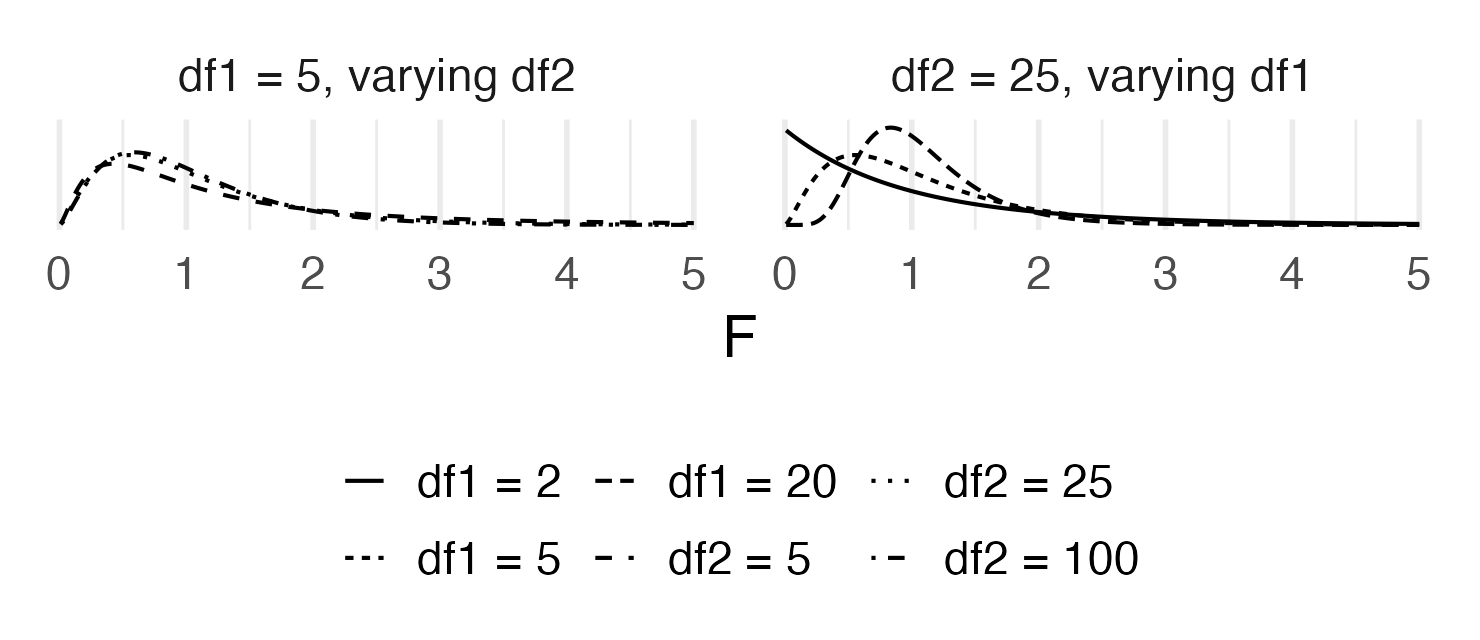
\includegraphics[width=0.92\textwidth]{f_shapes.png}
\end{center}

\vspace{0.2em}
{\small $df_1 = k - 1$ says how many groups; $df_2 = n - k$ says how much data. As $df_2$ grows the curve tightens around $1$, because more data pins down the within-group variance.}

\end{frame}


%%%%%%%%%%%%%%%%%%%%%%%%%%%%%%%%%%%%%%%%%%%%%%%%%%%%%%%%%%%%%%%%%%%%%%%%
\begin{frame}
\frametitle{The p-value is the right-hand tail}
\examplehead{PlantGrowth}

\vspace{-0.3em}
\begin{center}
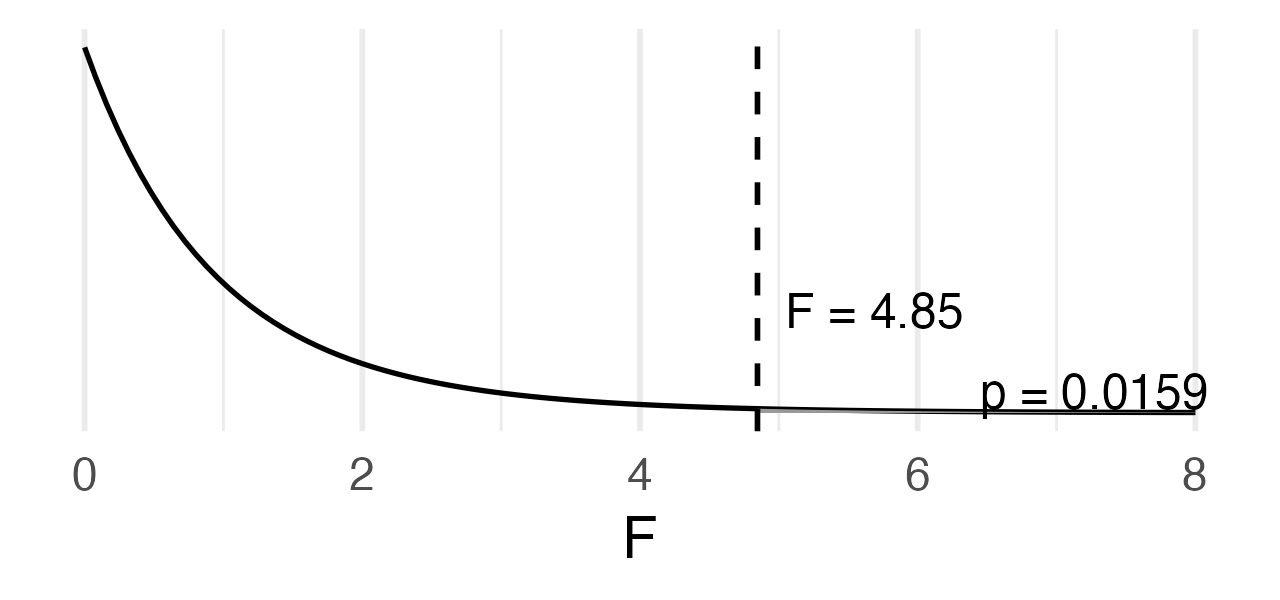
\includegraphics[width=0.7\textwidth]{f_tail.png}
\end{center}

\vspace{-0.3em}
{\small Only large $F$ argues against $H_0$, so the p-value is the $F_{2,27}$ area right of $4.85$: $\;P(F_{2,27} \ge 4.85) = \hl{0.0159}$.}

\vspace{-0.2em}
{\small In R, \texttt{pf(4.85, 2, 27, lower.tail = FALSE)}: exactly the $\Pr(>F)$ in the \texttt{aov} table.}

\end{frame}


%%%%%%%%%%%%%%%%%%%%%%%%%%%%%%%%%%%%%%%%%%%%%%%%%%%%%%%%%%%%%%%%%%%%%%%%
\begin{frame}
\frametitle{And the two roads agree}
\examplehead{PlantGrowth}

\vspace{-0.2em}
\begin{center}
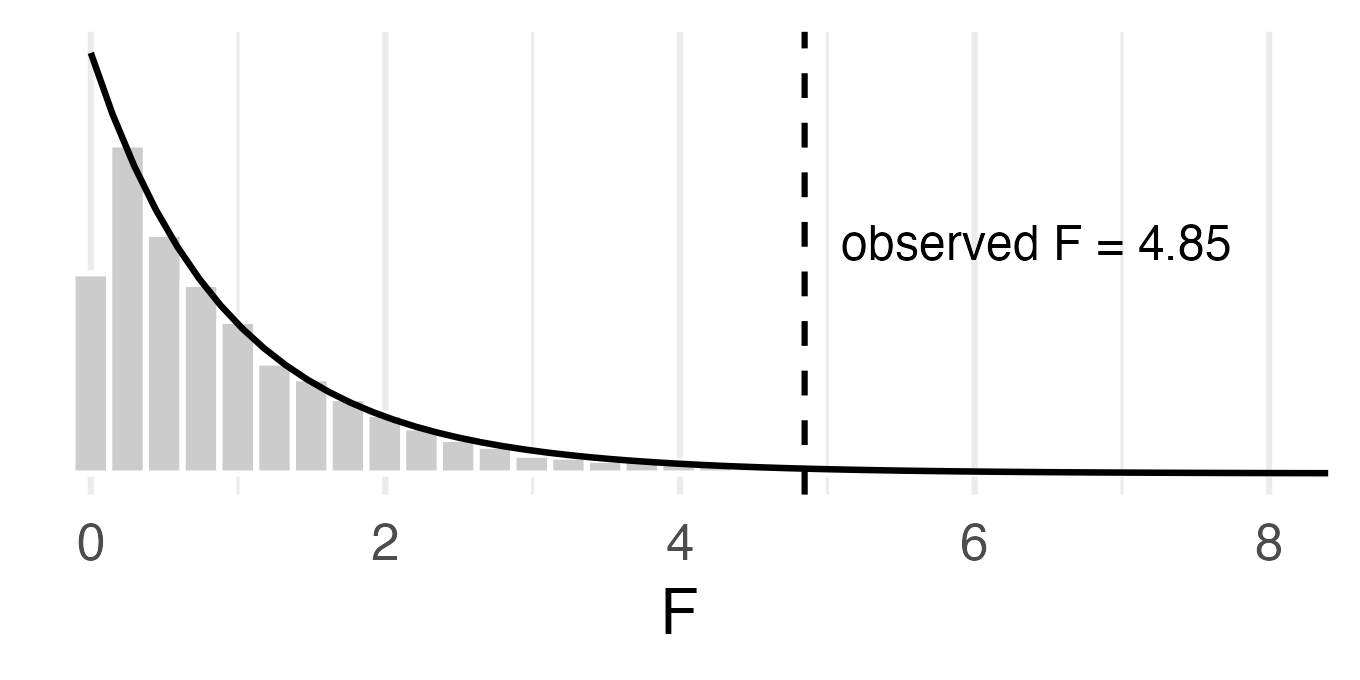
\includegraphics[width=0.66\textwidth]{f_vs_shuffle.png}
\end{center}

\vspace{-0.4em}
\keyidea{Shuffling gave $p = 0.0167$, the formula $p = 0.0159$. The $10{,}000$ shuffled $F$-values averaged $1.09$, and an $F_{2,27}$ has mean $\tfrac{27}{25} = 1.08$. \emph{That} is why we expect $F \approx 1$ under $H_0$.}

\end{frame}




\section{Conditions for the F-test}

%%%%%%%%%%%%%%%%%%%%%%%%%%%%%%%%%%%%%%%%%%%%%%%%%%%%%%%%%%%%%%%%%%%%%%%%
\begin{frame}
\frametitle{Road B has conditions; Road A has one}

The $F_{df_1,df_2}$ formula is a shortcut, and it is trustworthy only when:

\begin{enumerate}
\item \textbf{Independence:} observations do not influence one another (random sampling or assignment buys this).
\item \textbf{Approximate normality} within each group: matters most for small groups. Check a Q-Q plot.
\item \textbf{Equal variances:} as a rule of thumb, largest SD $<\;2\times$ smallest SD.
\end{enumerate}

\pause
\caution{Shuffling (Road A) looks assumption-free, but it needs \emph{exchangeability}: under $H_0$ any observation could carry any label. Condition 3 is exactly what makes that true, so it is not just Road B's problem.}

\end{frame}


%%%%%%%%%%%%%%%%%%%%%%%%%%%%%%%%%%%%%%%%%%%%%%%%%%%%%%%%%%%%%%%%%%%%%%%%
\begin{frame}
\frametitle{Checking the conditions on the plants}
\examplehead{PlantGrowth}

Look at the residuals ($x_{ij} - \bar{x}_i$, each plant minus its group mean):

\vspace{-0.3em}
\twocol{0.5}{0.5}
{
\begin{center}
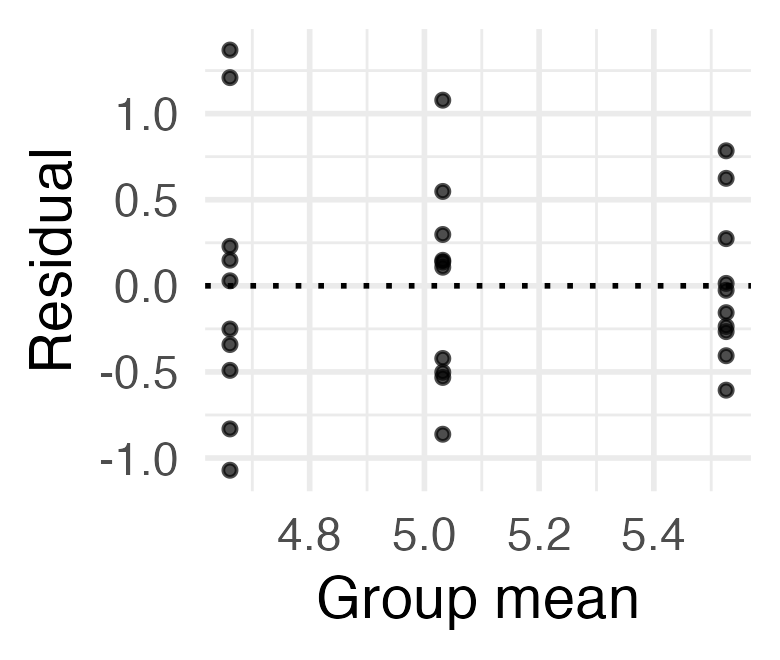
\includegraphics[width=0.82\textwidth]{anova_resid.png}
\end{center}
}
{
\begin{center}
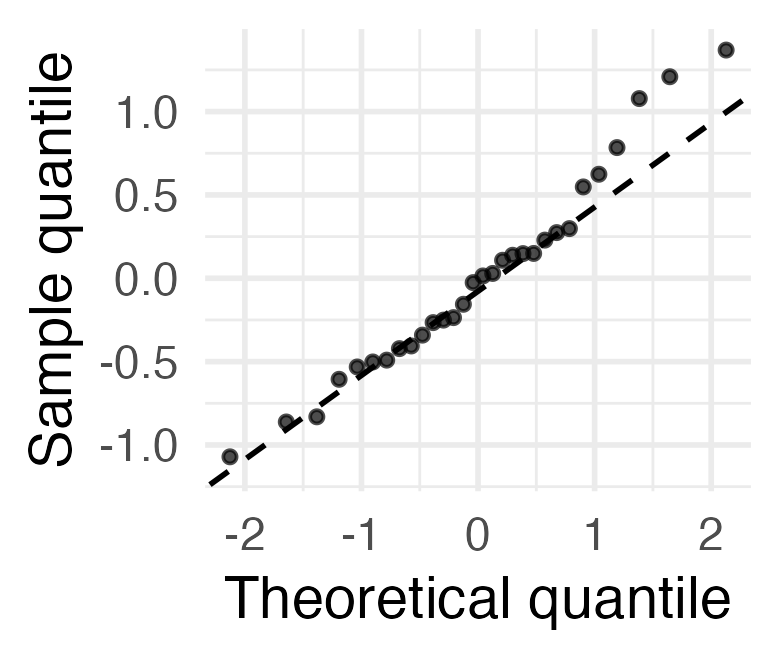
\includegraphics[width=0.82\textwidth]{anova_qq.png}
\end{center}
}

\vspace{-0.2em}
{\small \textbf{Left:} spread is about equal across columns (SDs $0.58$, $0.79$, $0.44$; ratio $1.8 < 2$). \textbf{Right:} residuals hug the line, so normality is reasonable. Both roads are entitled to run, \hl{which is why they agreed}.}

\end{frame}


%%%%%%%%%%%%%%%%%%%%%%%%%%%%%%%%%%%%%%%%%%%%%%%%%%%%%%%%%%%%%%%%%%%%%%%%
\begin{frame}
\frametitle{Does the equal-variance condition actually matter?}

\vspace{-0.3em}
\begin{center}
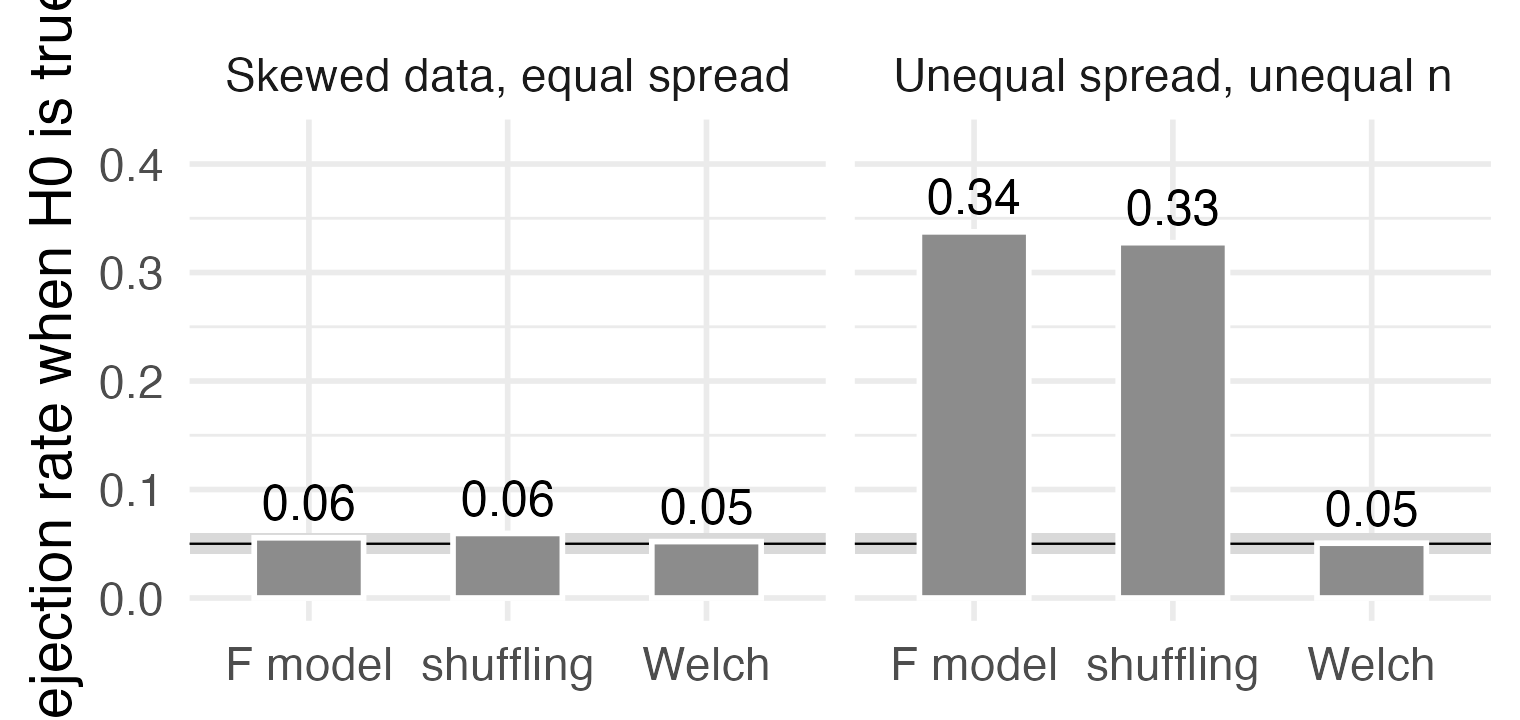
\includegraphics[width=0.82\textwidth]{anova_condition_check.png}
\end{center}

\vspace{-0.4em}
{\small We generated $2{,}000$ datasets in which $H_0$ was \emph{true} and counted how often each method rejected anyway. A working test should reject $5\%$ of the time.}

\end{frame}


%%%%%%%%%%%%%%%%%%%%%%%%%%%%%%%%%%%%%%%%%%%%%%%%%%%%%%%%%%%%%%%%%%%%%%%%
\begin{frame}
\frametitle{Shuffling is not a free pass}

\keyidea[-- read the right-hand panel]{%
\begin{itemize}\setlength{\itemsep}{1pt}
\item Skewed data, equal spreads: \emph{both} roads hold their $5\%$ rate. Non-normality alone is survivable.
\item Unequal spreads \emph{and} unbalanced groups: the $F$-test rejects $34\%$ of the time, \hl{and so does shuffling} ($33\%$).
\item Unequal variance breaks exchangeability, so Road A goes down with Road B.
\end{itemize}}

\pause
\vspace{0.3em}
{\small The fix for unequal variances is not permutation but \hl{Welch's ANOVA} (\texttt{oneway.test(y \textasciitilde{} g, var.equal = FALSE)}), which held its $5\%$ rate throughout. Shuffling buys you robustness to \emph{non-normality}, not to \emph{unequal variance}.}

\end{frame}


\section{After a significant F}

%%%%%%%%%%%%%%%%%%%%%%%%%%%%%%%%%%%%%%%%%%%%%%%%%%%%%%%%%%%%%%%%%%%%%%%%
\begin{frame}
\frametitle{A significant $F$: so \emph{which} groups differ?}
\examplehead{PlantGrowth}

$F$ only says ``at least one mean differs''. \texttt{TukeyHSD(fit)} compares every pair and corrects for testing all three:

\vspace{0.2em}
\begin{center}
{\small
\begin{tabular}{lcc}
\toprule
comparison & difference & adjusted $p$ \\
\midrule
\texttt{trt1 - ctrl} & $-0.37$ & $0.39$ \\
\texttt{trt2 - ctrl} & $+0.49$ & $0.20$ \\
\texttt{trt2 - trt1} & $+0.87$ & $\mathbf{0.012}$ \\
\bottomrule
\end{tabular}}
\end{center}

\pause
\keyidea{The overall test was significant, yet \emph{neither treatment beats the control}. All the signal is \texttt{trt2} vs \texttt{trt1}.}

\end{frame}


%%%%%%%%%%%%%%%%%%%%%%%%%%%%%%%%%%%%%%%%%%%%%%%%%%%%%%%%%%%%%%%%%%%%%%%%
\begin{frame}
\frametitle{$F$ is about \emph{means}, sometimes the wrong question}

\vspace{-0.3em}
\begin{center}
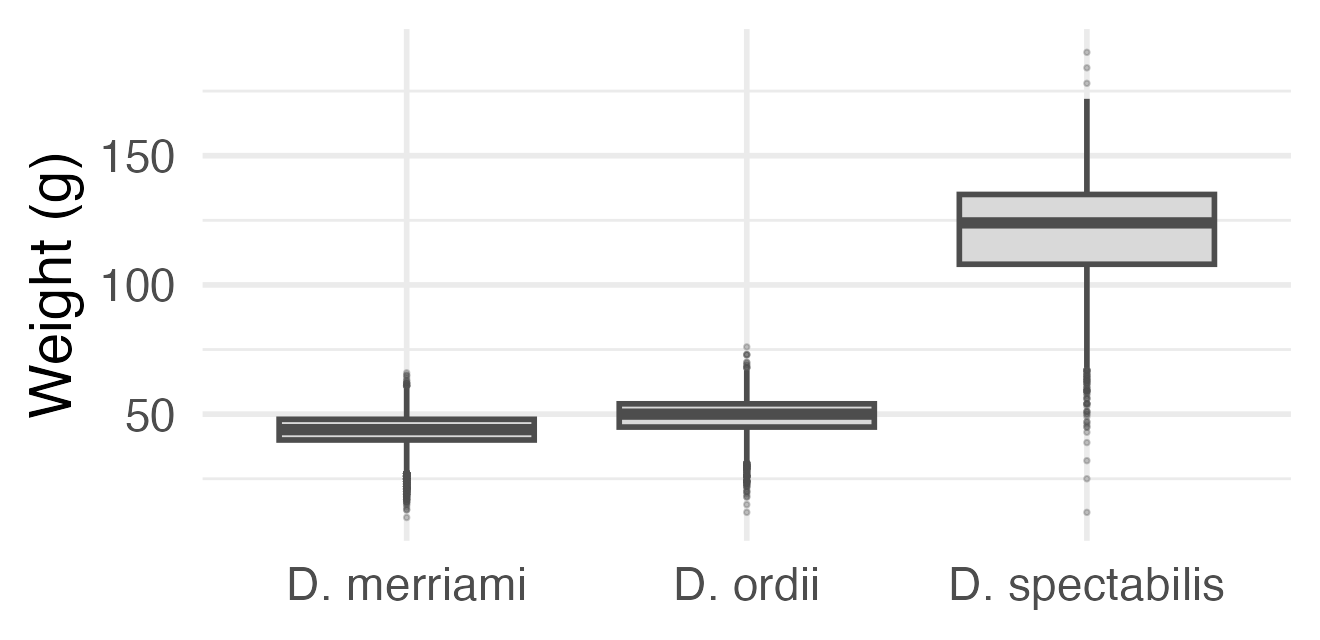
\includegraphics[width=0.64\textwidth]{portal_species.png}
\end{center}

\vspace{-0.3em}
{\small Three Portal kangaroo-rat species. \emph{D.\ spectabilis} is not just heavier. It is far more \hl{spread out} (SD $22.9$ vs $6.8$ and $7.9$). Equal variance fails badly, and the mean is dragged around by the long right tail.}

\end{frame}


%%%%%%%%%%%%%%%%%%%%%%%%%%%%%%%%%%%%%%%%%%%%%%%%%%%%%%%%%%%%%%%%%%%%%%%%
\begin{frame}
\frametitle{The real payoff of Road A: choose your own statistic}

The $F$ formula can only ever compare \emph{means}. Shuffling has no such limit: the recipe works for \hl{any} number you can compute:

\vspace{0.2em}
\begin{itemize}
\item a statistic built from group \hl{medians}, when outliers should not decide the verdict;
\item the Kruskal--Wallis statistic, built from \hl{ranks};
\item the largest pairwise gap, if that is what you care about.
\end{itemize}

\pause
\keyidea{That is why the two roads are not interchangeable even when they agree: the formula answers one fixed question about means; shuffling lets you \emph{choose the question} and still get a valid p-value.}

\end{frame}


\section{Wrap-up}

%%%%%%%%%%%%%%%%%%%%%%%%%%%%%%%%%%%%%%%%%%%%%%%%%%%%%%%%%%%%%%%%%%%%%%%%
\begin{frame}
\frametitle{Two roads, whatever the statistic}

{\scriptsize
\begin{center}
\setlength{\tabcolsep}{2.5pt}
\begin{tabular}{lll}
\toprule
\textbf{The statistic} & \textbf{By simulation} & \textbf{By formula} \\
\midrule
a proportion & simulate $H_0$ (Lec 8) & binomial, exact; $z$ (Lec 10) \\
a mean or a difference & bootstrap (Lec 9), permute (Lec 8) & the CLT: $z$, $t$ (Lec 10) \\
a whole table, $X^2$ & permute one column (Lec 11) & $\chi^2_{df}$ (Lec 11) \\
\hl{several group means, $F$} & \hl{permute the labels (today)} & \hl{$F_{df_1,df_2}$ (today)} \\
\bottomrule
\end{tabular}
\end{center}}

\vspace{0.3em}
The recipe never changed: \emph{state $H_0$, build a statistic, get its null distribution (by simulating $H_0$, or by a formula whose conditions hold), then ask how extreme the observed value is.}


\end{frame}


%%%%%%%%%%%%%%%%%%%%%%%%%%%%%%%%%%%%%%%%%%%%%%%%%%%%%%%%%%%%%%%%%%%%%%%%
\begin{frame}
\frametitle{Summary}

\begin{itemize}
\item Testing every pair inflates the error rate. ANOVA asks one question, \emph{are all $k$ means equal?}, with one $\alpha$.
\item $F = MSG/MSE$ weighs variability \hl{between} groups against variability \hl{within}. Near $1$ under $H_0$; large $F$ is evidence.
\item Two roads to its null distribution, \hl{shuffle the labels} or the \hl{$F_{df_1,df_2}$ model}, and they agreed ($p = 0.017$ vs $0.016$).
\item Both roads need \hl{equal variances}; normality alone matters far less. When variances differ, use \hl{Welch}.
\item A significant $F$ only says ``something differs''. Use Tukey for \emph{which}, and shuffling for statistics other than the mean.
\end{itemize}

\end{frame}


%%%%%%%%%%%%%%%%%%%%%%%%%%%%%%%%%%%%%%%%%%%%%%%%%%%%%%%%%%%%%%%%%%%%%%%%
\begin{frame}
\frametitle{Coming up next}

\hl{Next class, Module 3, inference for regression:} the statistic becomes a \emph{regression slope}. Is the line real, or could that tilt be noise? The same two roads return: permute, or a $t$ formula (IMS Ch.\ 24).

\vspace{0.4em}
\begin{itemize}
\item And $F$ is not done with us: every \texttt{lm()} summary ends with an $F$-statistic. When we reach multiple regression, that line is \emph{this} test.
\end{itemize}

\end{frame}


%%%%%%%%%%%%%%%%%%%%%%%%%%%%%%%%%%%%%%%%%%%%%%%%%%%%%%%%%%%%%%%%%%%%%%%%
% Activity
%%%%%%%%%%%%%%%%%%%%%%%%%%%%%%%%%%%%%%%%%%%%%%%%%%%%%%%%%%%%%%%%%%%%%%%%

\begin{frame}
\frametitle{Activity: does plot type change a rat's weight?}

\activity{In Lecture 11 you tested whether \emph{which species} you catch depends on plot type. Today, for \emph{D.\ merriami} alone:
\begin{itemize}\setlength{\itemsep}{1pt}
\item Does mean \hl{weight} differ across the five plot types?
\item Run the $F$-test \emph{and} the shuffle test.
\item Check the conditions, and see whether ``significant'' means ``large''.
\end{itemize}}

\vspace{0.3em}
{\small
\begin{itemize}
\item Work in \emph{pairs} (analyst + guide), one worksheet per pair.
\item We pause for check-ins. \hl{Be ready to share}.
\item Data and starter code are on Blackboard.
\end{itemize}}

\end{frame}



%%%%%%%%%%%%%%%%%%%%%%%%%%%%%%%%%%%%
% End document
%%%%%%%%%%%%%%%%%%%%%%%%%%%%%%%%%%%%

\end{document}
